\section{Browser Security Warnings and HTTPS Errors}
%����Ҫ��дһ���ܽ���ܵĻ�
\subsection{Browser Security Warnings}
Browser security warnings protect users against various network attacks,
    and this paper only considers the MitM attacks in HTTPS.
The  attacks might be launched
     by using a forged certificate,
    or deceiving browsers to visit the web server through HTTP.
When such HTTPS errors happen,
    a browser shows the warnings in different way to ensure security while minimize the side effects of user experience,
    because an HTTPS error is not definitely caused by a MitM attack.

% We describe security warnings of major browsers.

\subsubsection{Level A: Low-risk warning}
For low-risk errors, it shows a security indicator without interrupting the user's browsing.
For example,
    the browser removes the HTTPS lock icon, change the icon's color, or show a hint text.
%In this scenario, a passive security indicator indicates minor HTTPS errors by removing lock icon, changing lock icon��s color, providing textual information, or by other means without interrupting the user��s browsing.
%This is probably because webmaster has configured his website correctly, including purchasing a valid certificate, but the website still contains images or scripts over plain HTTP.
%Although the browser was able to establish a valid HTTPS connection, there are still minor problems.
On low-risk errors,
 the browser still establishes HTTPS connections with visited web server.

\begin{figure}[htb]
\centerline{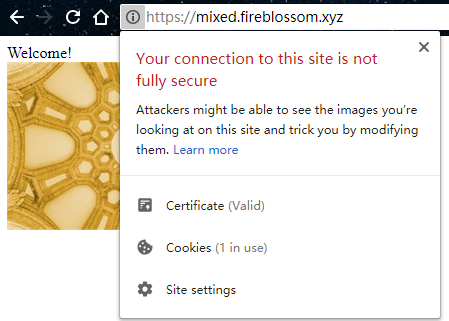
\includegraphics[height=3cm,width=7cm]{Figure/fig1.png}}%�ǵû���chrome�Ľ�ͼ
\caption{Low-risk warning in Chrome.}
\label{fig}
\end{figure}

\subsubsection{Level B: Medium-risk warning}
For medium-risk errors, it shows a bypassable warning that discourages the user from continuing.
For example,
    the browser stops the page load and display a full-screen warning with two options: "Click here to close this webpage" and "Continue to this website (not recommended)".
On medium-risk errors,
 the traffic is still encrypted between browser and web server, even if the user click through the warning.
%For medium-risk errors, it will show a bypassable warning that discourages the user from continuing.
%Bypassable HTTPS security warnings are the most common type of browser warning. Browsers use bypassable HTTPS security warning to treat the vast majority of HTTPS errors.
\begin{figure}[htb]
\centerline{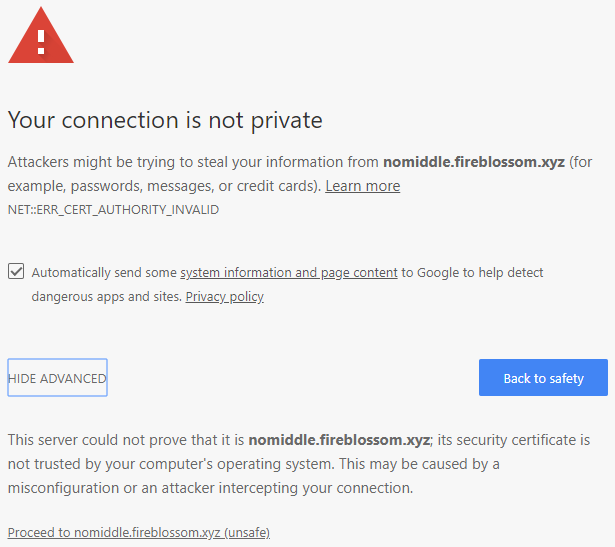
\includegraphics[height=3cm,width=7cm]{Figure/fig2.png}}
\caption{Medium-risk warning in Chrome.}
\label{fig}
\end{figure}
%In this scenario, if there is an HTTPS error, the browser will stop the page load and display an HTTPS security warning explaining the cause of the error. Typically, users are able to click through the warning by clicking on a button, but this may be disabled if the website servers the HTTP Strict Transport Security (HSTS) or HTTP Public Key Pinning (HPKP) header. Although the HTTP(s) traffic we captured through Fiddler[ https://www.telerik.com/fiddler] shows the web page is not transmitted in plain text, clicking through the warning may allow an actual man-in-the-middle attack to proceed.

\subsubsection{Level C: High-risk warning}
For high-risk errors, it shows a non-bypassable warning that stops the user from continuing.
For example, 
    the browser displays a full-screen warning explaining the cause of the error, and there is only a retry button to choose.
On high-risk errors,
    the browser refuses to establish an HTTPS connection to the server.
    
%For high-risk errors, it will show a security warning that the user cannot bypass.
%As a worst case scenario, the browser will prevent uses from continuing to browse the website by showing a security warning that the users cannot bypass.
\begin{figure}[htbp]
\centerline{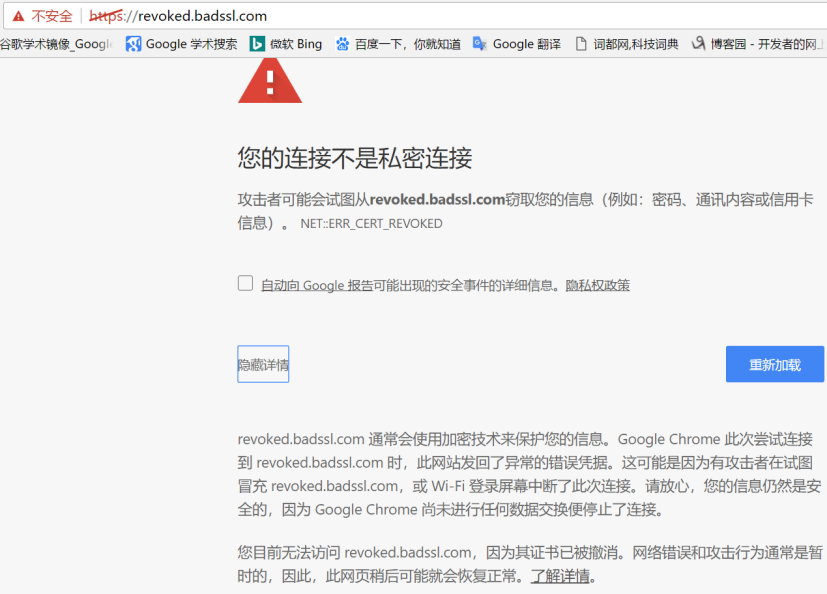
\includegraphics[height=3cm,width=7cm]{Figure/fig3.png}}%�ǵû����Լ�fireblossom.xyz��ַ�Ľ�ͼ
\caption{High-risk warning in Chrome.}
\label{fig}
\end{figure}
%this is probably because the website is supposed to establish a valid HTTPS connection, but the certificate chain fails to validate (e.g., a HTTPS certificate error occurs in a website that has deployed HSTS policy).

\subsubsection{Level D: Fatal warning}
secure connection failed
%For fatal errors, it shows a warning stop uses' browsing.
%On medium-risk errors, the browser cannot establish HTTPS connection with visited web server.
%The browser may fail to establish a HTTPS connection to the server for unsupported TLS version, cipher mismatch, or other reasons.
%In this scenario, the browser cannot obtain certificates from the web server, let alone certificate validation, so the TLS handshake error is not discussed in this paper.
\begin{figure}[htbp]
\centerline{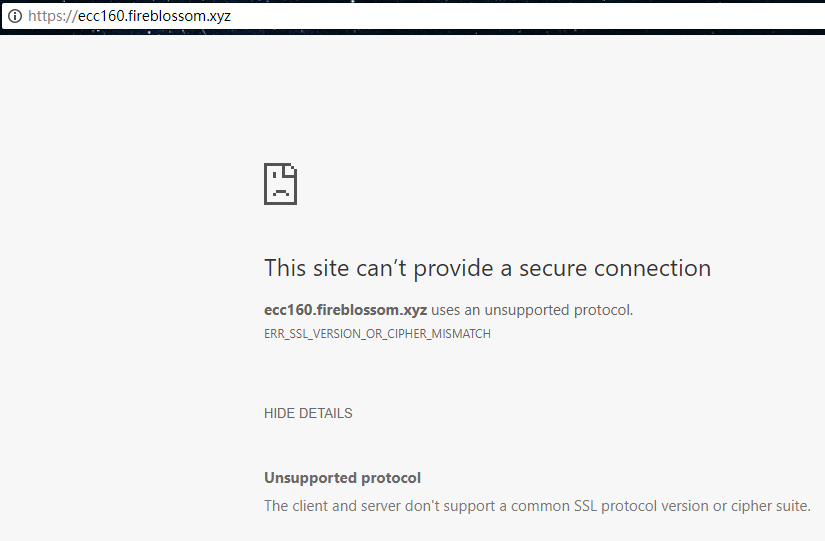
\includegraphics[height=3cm,width=7cm]{Figure/fig4.png}}%��ͼ��Ҫ�ٵ�����������
\caption{Fatal warning in Chrome.}
\label{fig}
\end{figure}
%Warning Images
